% !Mode:: "TeX:UTF-8"	% read in as utf8 file.

\chapter{Nonlinear}

\section{Non-linear partial equations of elasticity}
In solid mechanics, 3D deformable objects are modelled by the non-linear partial equations of elasticity. After applying FEM, one obtains an ordinary differential equation,

\begin{equation} \label{eq: fem_ode}
	\mathbf{M}\ddot{\mathbf{u}}+\mathbf{D}\dot{\mathbf{u}}+\mathbf{f}_{\mathrm{int}}(\mathbf{u})=\mathbf{f}_{\mathrm{ext}}(t)
\end{equation}

where:
\begin{itemize}
	\item $ \mathbf{M}\in \mathbb{R}^{3n\times 3n} $ is the mass matrix;
	\item $ \mathbf{u}\in \mathbb{R}^{3n} $ contains the displacements of the $ n $ mesh vertices away from the rest configuration;
	\item $ \mathbf{D}=\alpha \mathbf{M}+\beta \mathbf{M}(\mathbf{u})+\bar{\mathbf{D}} $ is the damping matrix. Scalar $ \alpha $ and $ \beta $ and matrix $ \bar{\mathbf{D}} \in \mathbb{R}^{3n \times 3n} $ control damping: $ \alpha $ sets the level of 'mass' damping(slows down deformations globally, as in underwater damping), $ \beta $ sets the 'stiffness' damping(damps primarilly any relative deformation velocity differences; useful to remove temporal high-frequency instabilities) and $ \bar{\mathbf{D}} $ is an additional damping matrix that can optionally be set by the user. For $ \bar{\mathbf{D}} = 0 $, we obtain the familiar Rayleigh damping;
	\item $ \mathbf{f}_{\mathrm{int}}(\mathbf{u})\in \mathbb{R}^{3n} $ are the internal elastic forces. The gradient of $ \mathbf{f}_{\mathrm{int}}(\mathbf{u}) $ with respect to $ \mathbf{u} $, $ \mathbf{K}(\mathbf{u})=\partial \mathbf{f}_{\mathrm{int}}(\mathbf{u})/\partial \mathbf{u} \in \mathbb{R}^{3n\times 3n} $ is called the tangent stiffness matrix;
	\item $ \mathbf{f}_{\mathrm{ext}}(t) \in \mathbb{R}^{3n} $ are external forces(e.g. gravity, wind, contact, user forces)
\end{itemize}

\section{Deformation map and deformation gradient}
Our initial objective is to provide a concise mathematical description of the deformation that an elastic body has sustained. This formulation will lay the foundation for appropriate representations of other physical properties such as \textbf{force} and \textbf{energy}.

The relation between each material point and its respective deformed location is captured by the \textit{deformation function} $ \vec{\phi}: \mathbf{R}^3 \rightarrow \mathbf{R}^3 $ which maps every material point $ \vec{X} $ to its respective deformed location $ \vec{x}=\vec{\phi} (\vec{X}) $.

An important physical quantity derived directly from $ \vec{\phi} (\vec{X}) $, whose utility will become apparent in the next section, is the \textit{deformation gradient} tensor $ \mathbf{F} \in \mathbf{R}^{3\times 3} $. If we write $ \vec{X}=(X_1,X_2,X_3)^T $ and $ \vec{\phi} (\vec{X}) = \left( \phi _1(\vec{X}),\phi _2(\vec{X}), \phi _3(\vec{X}) \right)^T $ for the three components of the vector-valued function $ \vec{\phi} $, the deformation is written as:
\begin{equation}
	\mathbf{F:=\dfrac{\partial (\phi _1,\phi _2, \phi _3)}{\partial (X_1, X_2,X_3)}=\left( 
		\begin{matrix}
			\dfrac{\partial \phi _1}{\partial X_1} & \dfrac{\partial \phi _1}{\partial X_2} & \dfrac{\partial \phi _1}{\partial X_3}\\
			\dfrac{\partial \phi _2}{\partial X_1} & \dfrac{\partial \phi _2}{\partial X_2} & \dfrac{\partial \phi _2}{\partial X_3}\\
			\dfrac{\partial \phi _3}{\partial X_1} & \dfrac{\partial \phi _3}{\partial X_2} & \dfrac{\partial \phi _3}{\partial X_3}\\
		\end{matrix} \right)}
\end{equation}

or, in index notation $ F_{ij}=\phi _{i,j} $. That is, $ \mathbf{F} $ is the \textbf{Jacobian matrix} of the deformation map.

\section{Tangent Stiffness Matrix}
The nonlinear system of equations are expressed simply as:

\begin{equation} \label{eq: residual forces}
\mathbf{r}(x) = \mathbf{f}_\mathrm{ext}(\mathbf{x}) - \mathbf{f}_\mathrm{int}(\mathbf{x}) = \mathbf{0}
\end{equation}

This is solved using a Newton-Raphson scheme.  Equation \ref{eq: residual forces} is expressed as a truncated Taylor series expansion, whereby the residual $ \mathbf{r} $ at the next iteration is expressed as:

\begin{equation}
\mathbf{r}_{i+1} = \mathbf{r}_i + \dfrac{\partial \mathbf{r}_i}{\partial \mathbf{x}} d\mathbf{x}
\end{equation}

where
\begin{equation}
\dfrac{\partial \mathbf{r}_i}{\partial \mathbf{x}} = -\dfrac{\mathbf{f}_\mathrm{int}(\mathbf{x})}{\partial \mathbf{x}} = -\mathbf{K}_t = -\int_{V} \mathbf{B}^T\dfrac{\partial \mathbf{P}}{\partial \mathbf{F}} \mathbf{B} dV
\end{equation}

The derivative $ \dfrac{\partial \mathbf{P}}{\partial \mathbf{F}} $ is the elasticity tensor $ \mathbf{C} $.

\section{Implicit backward Euler} \label{App: implicit backward euler}

With an ordinary differential equation:

\begin{equation}
	\mathbf{M}\ddot{\mathbf{u}}+\mathbf{D}\dot{\mathbf{u}}+\mathbf{f}_{\mathrm{int}}(\mathbf{u})=\mathbf{f}_{\mathrm{ext}}(t)
\end{equation}

Given deformation $ \mathbf{u}_t $ and velocity $ \mathbf{v}_t $ at time $ t $, the implicit backward Euler method attempts to find a future deformation $ \mathbf{u}_{t+\Delta t} $ such that explicitly integrating at time $ t $ with forces $ \mathbf{f}_{\mathrm{int}(\mathbf{u}_{t+\Delta t})} $ evaluated at $ t+\Delta t $ will produce the same deformation $ \mathbf{u}_{t+\Delta t} $. If we let $ \Delta \mathbf{u} = \mathbf{u}_{t+\Delta t}-\mathbf{u}_t $ and $ \Delta \mathbf{v} = \mathbf{v}_{t+\Delta t}-\mathbf{v}_t $ represent the changes in deformation and velocity from time $ t $ to $ t+\Delta t $, then we want to set

\begin{equation} \label{eq: Implicit nolinear backward euler}
	\left[ \begin{array}{c}
		\Delta \mathbf{u} \\
		\Delta \mathbf{v}
	\end{array} \right] = \Delta t \left[ \begin{array}{l}
	\Delta \mathbf{v}+\mathbf{v}_t \\
	\mathbf{M}^{-1}\left( -\mathbf{D}\mathbf{v}_{t+\Delta t}-\mathbf{f}_{\mathrm{int}}(\mathbf{u}_{t+\Delta t})+\mathbf{f}_{\mathrm{ext}}\right) 
\end{array} \right]
\end{equation}

Replace $ f_\mathrm{int}(\mathbf{u}_{t+\Delta t}) $ with $ \mathbf{M}(\mathbf{u}_t+\Delta \mathbf{u}) $ and add $ \mathbf{M}\mathbf{v}_t $ to both sides of equation \ref{eq: Implicit nolinear backward euler}, and notice that $ \Delta \mathbf{u} = \delta t \times \mathbf{v}_{t+\Delta t} $, we have

\begin{equation} \label{Implicit linear backward euler}
	\left(\mathbf{M}+\Delta t\mathbf{D}+(\Delta t)^2\mathbf{K}\right)\mathbf{v}_{t+\Delta t} = \mathbf{M}\mathbf{v}_t + \Delta t\left(\mathbf{f}_{\mathrm{ext}}-\mathbf{K}\mathbf{u}_t\right)
\end{equation}

After solving Equation \ref{Implicit linear backward euler} for $ \mathbf{v}_{t+\Delta t} $, we can calculate $ \Delta \mathbf{u} $ from Equation \ref{eq: Implicit nolinear backward euler}.

\section{Conjugate Gradient Solver} \label{App: conjugate gradient solver}
\url{Quote from: http://en.wikipedia.org/wiki/Conjugate_gradient_method}

In mathematics, the \textbf{conjugate gradient } is an algorithm for the numerical solution of particular systems of linear equations, namely those whose matrix is \textbf{symmetric} and \textbf{positive-definite}. The conjugate gradient method is often implemented as an iterative algorithm, application to sparse systems that are too large to be handled by a direct implementation or other direct methods such as \textbf{Cholesky decomposition}. Large sparse systems often arise when numerically solving \textbf{partial differential equations} or optimization problems.

The conjugate gradient method can also be used to solve unconstrained optimization problems such as energy minimization. It was mainly developed by Magnus Hestenes and Eduard Stiefel.

\begin{figure}[h]
	\centering
	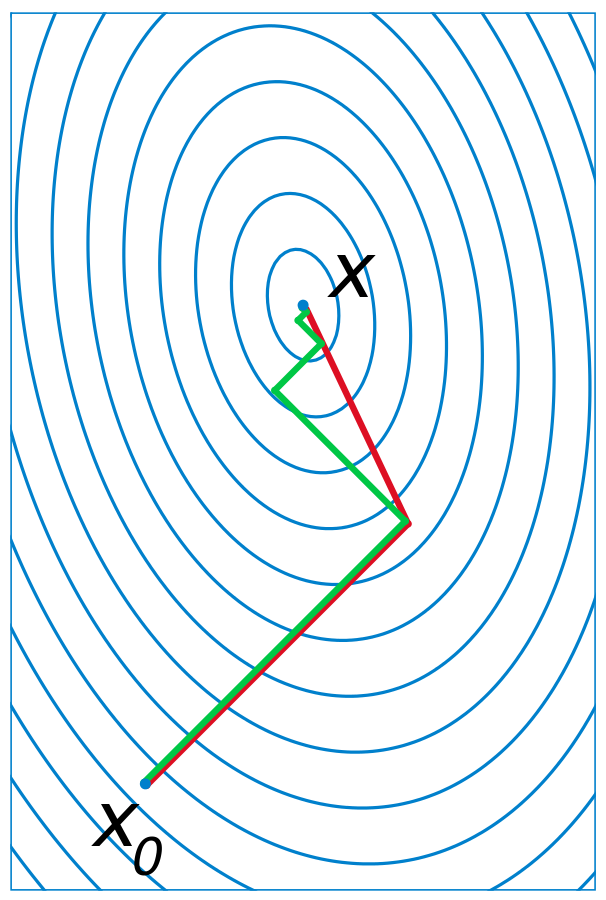
\includegraphics[width = 0.5\linewidth]{{figure/Conjugate_gradient_illustration.svg}.png}
\end{figure}

\subsection{Pseudocode}
The algorithm is detailed below for solving $ \mathbf{Ax = b} $ where $ \mathbf{A} $ is a real, symmetric, positive-define matrix. The input vector $ \mathbf{x_0} $  can be an approximate initial solution or $ \mathbf{0} $. It is a different formulation of the exact procedure described above.\\

\begin{eqnarray*}
	\mathbf{r}_0 &:=& \mathbf{b-A_0},\\
	\mathbf{p_0} &:=& \mathbf{r_0},\\
	k &:=& 0,\\
\end{eqnarray*}

\begin{flalign}
	x &= abcd & \\
	&= abcd + efgh
\end{flalign}

\section{Strain energy and hyperelasticity}
One of the consequences of elastic deformation is the accumulaton of potential energy in the deformed body which is referred to as \textbf{strain energy} in the context of deformble solids.


We have assumed that potential energy associated with a deformed configuration only depends on the final deformed shape, and not on the deformation path over time that brought the body into its current configuration. The independence of the strain energy on the prior deformation history is a characteristic property of so-called \textit{hyperelastic} materials ( which is the only class of materials we will address in this course). This property of this closely related with the fact that elastic forces of hyperelastic materials are \textit{conservative}: the total work done by the internal elastic forces in a deformation path depends solely on the initial and final configurations, not the path itself.

Different parts of a deforming body undergo shape changes of different severity. As a consequence, the relation between deformation and strain energy is better defined on a local scale. We achieve that by introducing an \textit{energy density} function $ \Psi [\phi; \vec{X}] $ which measures the strain energy \textit{per unit undeformed volume} on an infinitesimal domain $ dV $ around the material point $ \vec{X} $. We can then obtain the total energy for the deforming body by integrating the energy density function over the entire domain $ \Omega $:
\begin{equation*}
	E[\phi] = \int_{\Omega}{\Psi[\phi;\vec{X}]d\vec{X}}
\end{equation*}

Let us focus on a specific material location $ \vec{X}_* $. Since the energy density $ \Psi[\phi ; \vec{X}_*] $ would only need to reflect the deformation behavior in an infinitesimal neighborhood of $ \vec{X}_* $, we can reasonably approximate the deformation map in this tiny region using a first-order Taylor expansion:
\begin{equation*}
	\phi (\vec{X}) \approx \phi (\vec{X}_*) + \dfrac{\partial \phi}{\partial \vec{X}}\biggr\rvert_{\vec{X}_*}(\vec{X}-\vec{X}_*) = \vec{x}_*+\mathbf{F}(\vec{X}_*)(\vec{X}-\vec{X}_*)= \underbrace{\mathbf{F} (\vec{X}_*)}_{\mathbf{F}_*}\vec{X}+ \underbrace{\vec{x}_*-\mathbf{F}(\vec{X}_*)\vec{X}_*}_{\vec{t}}= \mathbf{F}_*\vec{X}+\vec{t}
\end{equation*}

This equation suggests that $ \Psi[\phi;\vec{X}_*] $ should be expressible as a function of $ \mathbf{F}_* $ and $ \vec{t} $, as these values fully parameterize the local Taylor approximation of $ \phi $ near $ \vec{X}_* $. Furthermore, we can expect that the value of the vector $ \vec{t} $ would be irrelevant in this expression: different values of this parameter would indicate deformations that differ only by a constant translation, thus producing the same deformed shape and the same strain energy. Thus, we expect that energy density function should be expressible as $ \Psi[\phi;\vec{X}] = \Psi (\mathbf{F} (\vec{X})) $, i.e. a function of the local deformation gradient alone.

\section{Abaqus explicit load increment method}
[Abaqus 6.10 \url{https://www.sharcnet.ca/Software/Abaqus610/Documentation/docs/v6.10/books/gsk/default.htm?startat=ch08s02.html}]

An increment is part of a step. In nonlinear analyses the total load applied in a step is broken into smaller increments sot that the nonlinear solution path can be followed.

\subsection{Equilibrium iterations and convergence in Abaqus/Standard}
The nonlinear response of a structure to a small load increment, $ \Delta P $, is shown in Figure \ref{fig:first_iteration_in_an_increment}. Abaqus/Standard uses the structure's initial stiffness, $ K_0 $, which is based on its configuration at $ u_0 $, and $ \Delta P $ to calculate a displacement correction, $ c_a $, for the structure. Using $ c_a $, the structure's configuration is updated to $ u_a $.

\begin{figure}[h]
\centering
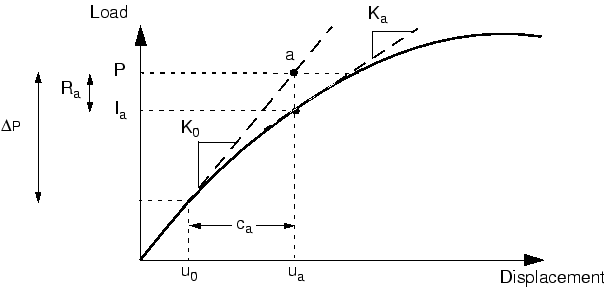
\includegraphics[width=0.7\linewidth]{figure/first_iteration_in_an_increment}
\caption{first iteration in an increment}
\label{fig:first_iteration_in_an_increment}
\end{figure}

\textbf{Convergence}

Abaqus/Standard forms a new stiffness, $ K_a $, for the structure, based on its updated configuration, $ u_a $. Abaqus/Standard also calculates $ I_a $, in this updated configuration. The difference between the total applied load, $ P $, and $ I_a $ can now be calculated as:

\begin{equation}
R_a = P - I_a
\end{equation}

If $ R_a $ is zero at every degree of freedom in the model, point $ a $ in Figure \ref{fig:first_iteration_in_an_increment} would lie on the load-deflection curve, and the structure would be in equilibrium. In a nonlinear problem it is almost impossible to have $ R_a $ equal to zero, so Abaqus/Standard compares it to a tolerance value. If $ R_a $ is less than this force residual tolerance, Abaqus/Standard accepts the structure's updated configuration as the equilibrium solution. By default, this tolerance value is set to \SI{0.5}{\percent} of an average force in the structure, averaged over time. Abaqus/Standard automatically calculates this spatially and time-averaged force throughout the simulation.

If $ R_a $ is less than the current tolerance value, $ P $ and $ I_a $ are in equilibrium, and $ u_a $ is a valid equilibrium configuration for the structure under the applied load. However, before Abaqus/Standard accepts the solution, it also checks that the displacement correction, $ c_a $, is small relative to the total incremental displacement, $ \Delta u_a = u_a 0 u_0 $. If $ c_a $ is greater than \SI{1}{\percent} of the increment displacement, Abaqus/Standard performs another iteration. Both convergence checks must be satisfied before a solution is said to have converged for that load increment. The exception to this rule is the case of a linear increment, which is defined as any increment in which the largest force residual is less than \num{e-8} times the time-averaged force. Any case that passes such a stringent comparison of the largest force residual with the time-averaged force is considered linear and does not require further iteration. The solution is accepted without any check on the size of the displacement correction.

If the solution form an iteration is not converged, Abaqus/Standard performs another iteration to try to bring the internal and external forces into balance. This second iteration uses the stiffness, $ K_a $, calculated at the end of the previous iteration together with $ R_a $ to determine another displacement correction, $ c_b $, that brings the system closer to equilibrium. (point $ b $ in figure \ref{fig:second_iteration}.

\begin{figure}[h]
\centering
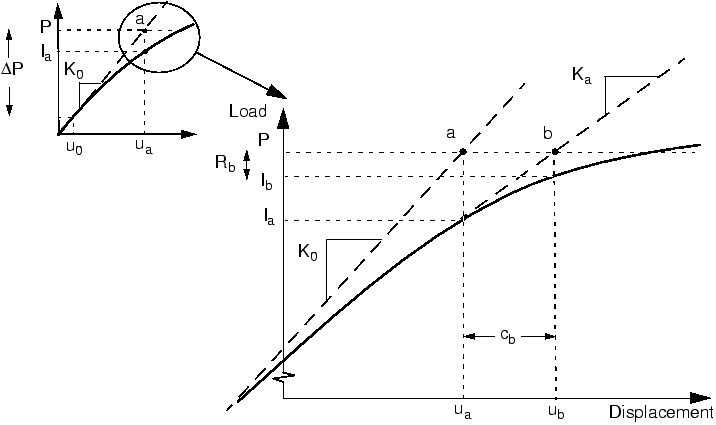
\includegraphics[width=0.7\linewidth]{figure/second_iteration}
\caption{second iteration}
\label{fig:second_iteration}
\end{figure}

Abaqus/Standard calculates a new force residual, $ R_b $, using the internal forces from the structure's new configuration, $ u_b $. Again, the largest force residual at any degree of freedom, $ R_b $, is compared against the force residual tolerance, and the displacement correction for the second iteration, $ c_b $, is compared to the increment of displacement, $ \Delta u_b = u_b-u_0 $. If necessary, Abaqus/Standard performs further iterations.

For each iteration in a nonlinear analysis Abaqus/Standard forms the model's stiffness matrix and solves a system of equations. This means that each iteration is equivalent, in computational cost, to conducting a complete linear analysis. It should now be clear that the computational expense of a nonlinear analysis in Abaqus/Standard can be many times greater than for a linear one.

It is possible with Abaqus/Standard to save results at each converged increment. Thus, the amount of output data available from a nonlinear simulation is many times that available from a linear analysis of the same geometry. Consider both of these factors and the types of nonlinear simulations that you want to perform when planning your computer resources.
